\section{Cognitive Variables}
\label{sec:cog}

IQ is measured for all individuals in the sample as well as for the caregivers of the children, migrants, and adolescents using Raven's Progressive Matrices (Raven's).\footnote{\citet{Raven_Raven_etal_1988_BOOKManualRavensprogressive}.} Raven's is a non-verbal test that is correlated with other measures of fluid intelligence. The 12-Item and 18-Item versions are shortened from the original version, which helps reduce the duration of the test. Both shortened versions are highly correlated with the full version of the test, which in turn is highly correlated with other measures of IQ.

Each item on the test consists of a matrix of diagrams that follow some logical pattern with one missing diagram that the test-taker needs to select from multiple choices. A correct answer is assigned a value of 1, and an incorrect answer is assigned a value of 0. The IQ score is the proportion of questions answered correctly. If questions are missed, then they do not count in the total number of questions. The factor scores are computed using a specification of a structural equation using maximum likelihood that accounts for missing values. That is, it requires the assumption that bot the observed and latent variables are jointly distributed normally, and that any missing values are missing at random. The latter assumption is the more tenuous assumption given that a missing item could mean the individual could not answer the question at all due to lower cognitive ability (as opposed to rushing through the test or inability to focus).
% The variables that measure these binary item-level responses for subjects are IQ*. For caregivers, the analogous variables are cgIQ*.

 Table \ref{tab:test-type} explains which individuals in which cohort received the 12- or 18-Item version of Raven's Progress Matrices (Raven's).

\begin{table}[htbp]
\begin{center}
	\caption{IQ Test by Cohort}\label{tab:test-type}
	\begin{tabular}{lcc}
		\toprule
		Cohort & 12-Item & 18-Item \\
		\midrule
		\textbf{Children} & &\\
		\quad Subjects & & $\checkmark$  \\
		\quad Caregivers &  $\checkmark$ & \\
		\textbf{Migrants} & & \\
		\quad Subjects & & $\checkmark$ \\
		\quad Caregivers & $\checkmark$ &  \\
		\textbf{Adolescents} & & \\
		\quad Subjects & $\checkmark$ & \\
		\quad Caregivers &  $\checkmark$ &  \\
		\textbf{Adults} & & \\
		\quad Subjects & & $\checkmark$ \\
		\bottomrule
	\end{tabular}
\end{center}
\raggedright \footnotesize Note: This table shows the type of test given for each cohort. The caregivers were always given the 12-Item Raven's. The 18-Item Raven's was only meant for younger subjects (the individuals in the children and migrants cohorts were about 6 years old at the time of the test).
\end{table}

Figure \ref{fig:iq-hist} shows the distribution of the IQ score by city and cohort. 

\begin{figure}[htbp]
	\begin{center}
	\caption{Densities of IQ Scores}\label{fig:iq-hist}
	\begin{subfigure}{.5\textwidth}
		\centering
		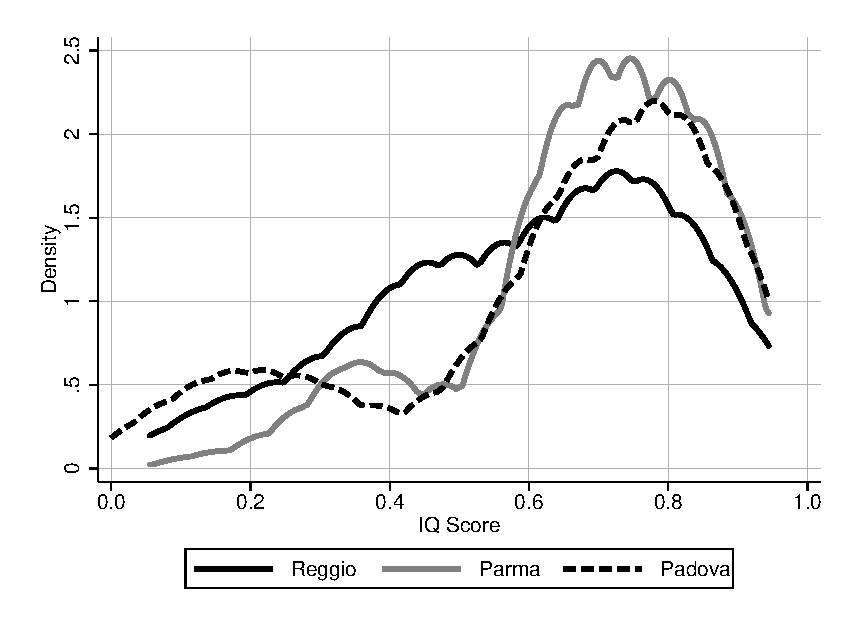
\includegraphics[width=20em]{../../../../Output/IQ_hist_1}
		\caption{Children}
	\end{subfigure}%
	\begin{subfigure}{.5\textwidth}
		\centering
		\includegraphics[width=20em]{../../../../Output/IQ_hist_2}
		\caption{Migrants}
	\end{subfigure}
	\begin{subfigure}{.5\textwidth}
		\centering
		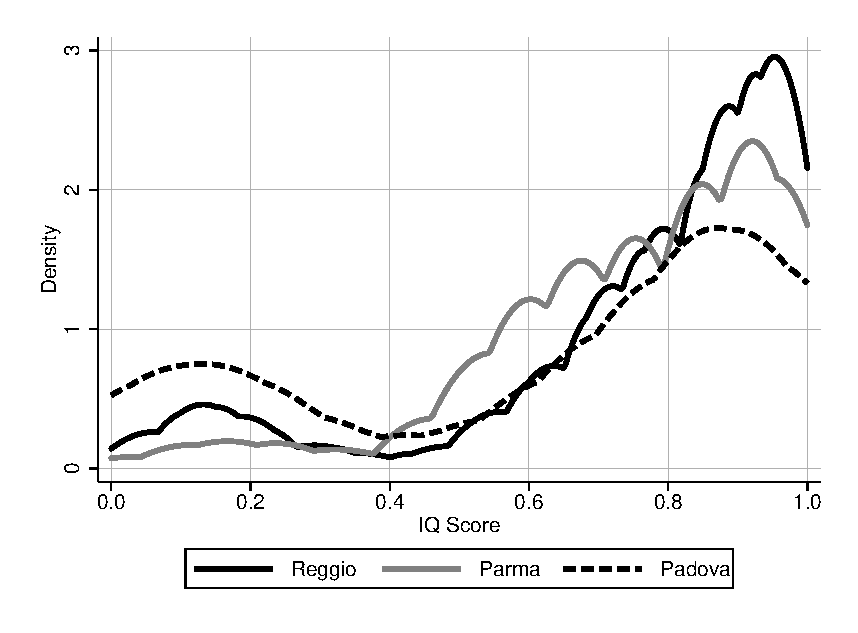
\includegraphics[width=20em]{../../../../Output/IQ_hist_3}
		\caption{Adolescents}
	\end{subfigure}%
	\begin{subfigure}{.5\textwidth}
		\centering
		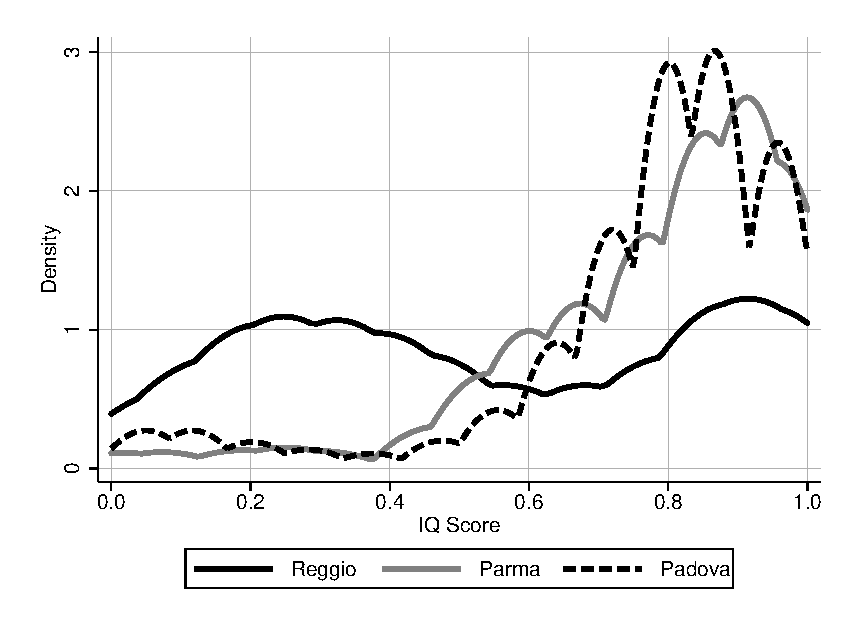
\includegraphics[width=20em]{../../../../Output/IQ_hist_4}
		\caption{Adults 30s}
	\end{subfigure}
	\begin{subfigure}{.5\textwidth}
		\centering
		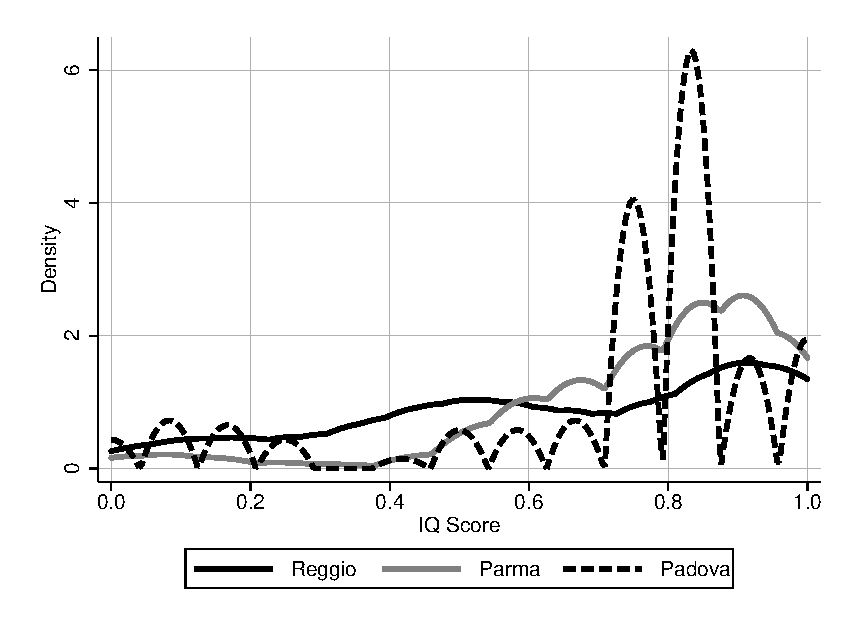
\includegraphics[width=20em]{../../../../Output/IQ_hist_5}
		\caption{Adults 40s}
	\end{subfigure}%
	\begin{subfigure}{.5\textwidth}
		\centering
		\includegraphics[width=20em]{../../../../Output/IQ_hist_6}
		\caption{Adults 50s}
	\end{subfigure}
\end{center}
\raggedright \footnotesize
Note: These plots show the distributions of IQ scores by city and cohort. The distributions of the different cities are more similar for the younger cohorts than for the adult cohorts. 
\end{figure}
